% !TEX TS-program = pdflatex
% !TEX encoding = UTF-8 Unicode

% This is a simple template for a LaTeX document using the "article" class.
% See "book", "report", "letter" for other types of document.

\documentclass[12pt]{article} % use larger type; default would be 10pt

\usepackage[utf8]{inputenc} % set input encoding (not needed with XeLaTeX)

%%% Examples of Article customizations
% These packages are optional, depending whether you want the features they provide.
% See the LaTeX Companion or other references for full information.

%%% PAGE DIMENSIONS
\usepackage{geometry} % to change the page dimensions
\geometry{letterpaper} % or letterpaper (US) or a5paper or....
% \geometry{margin=1in} % for example, change the margins to 2 inches all round
% \geometry{landscape} % set up the page for landscape
%   read geometry.pdf for detailed page layout information

\usepackage{graphicx} % support the \includegraphics command and options

% \usepackage[parfill]{parskip} % Activate to begin paragraphs with an empty line rather than an indent

%%% PACKAGES
\usepackage{booktabs} % for much better looking tables
\usepackage{array} % for better arrays (eg matrices) in maths
\usepackage{paralist} % very flexible & customisable lists (eg. enumerate/itemize, etc.)
\usepackage{verbatim} % adds environment for commenting out blocks of text & for better verbatim
\usepackage{subfig} % make it possible to include more than one captioned figure/table in a single float
\usepackage{amsmath}
% These packages are all incorporated in the memoir class to one degree or another...

%%% HEADERS & FOOTERS
\usepackage{fancyhdr} % This should be set AFTER setting up the page geometry
\pagestyle{fancy} % options: empty , plain , fancy
\renewcommand{\headrulewidth}{0pt} % customise the layout...
\lhead{}\chead{}\rhead{}
\lfoot{}\cfoot{\thepage}\rfoot{}

%%% SECTION TITLE APPEARANCE
\usepackage{sectsty}
\allsectionsfont{\sffamily\mdseries\upshape} % (See the fntguide.pdf for font help)
% (This matches ConTeXt defaults)

%%% ToC (table of contents) APPEARANCE
\usepackage[nottoc,notlof,notlot]{tocbibind} % Put the bibliography in the ToC
\usepackage[titles,subfigure]{tocloft} % Alter the style of the Table of Contents
\renewcommand{\cftsecfont}{\rmfamily\mdseries\upshape}
\renewcommand{\cftsecpagefont}{\rmfamily\mdseries\upshape} % No bold!

%%% END Article customizations

%%% The "real" document content comes below...

\title{Introduction to Macroeconomics and GDP}
\author{Abdon Morales \\ The University of Texas at Austin \\ ECO 304L: Intro to Macroeconomics}
%\date{today} % Activate to display a given date or no date (if empty),
         % otherwise the current date is printed 

\begin{document}
\maketitle

\section*{Big Questions}
\begin{center}
\begin{enumerate}
	\item How is macroeconomics different from microeconomics?
	\item How is GDP computed?
	\item What does GDP tell us about the economy?
	\item What are some shortcomings of GDP data?
\end{enumerate}
\end{center}

\section{Macroeconomics vs. Microeconomics}
\textbf{Macroeconomics} is the study of the economy as a whole. For exmaple, economic growth, unemployment, inflation, and etc.\\
\textbf{Microeconomics} is the study of decision-making by individuals and firms along how the government influences those decisions.

\section{GDP measures total production}
\begin{itemize}
	\item Gross Domestic Product is the market value of all final goods and services produced within a country during a specified period of time.
	\item It is the sum of the output from all (legal) economic activity.
\end{itemize}

\section{Circular Flow}

\includegraphics[scale=1]{../images/Screenshot 2024-01-22 at 12.57.43 AM.png} 

\section{What GDP measures}
\subsection{Gross Domestic Product}
\begin{itemize}
	\item The market value of all final goods and services produced in a country during a specific period of time.
\end{itemize}
\subsection*{Important notes}
\begin{itemize}
	\item Includes only final goods and services
	\item Includes only current production
	\item Does not include transfer payments
\end{itemize}
\subsubsection*{Counts in the market value}
\begin{itemize}
	\item{Suppose the country of Gondor produces the following: 10 oranges, 15 cloaks, and 6 swords}
	\item{Would it make sense to add them up to get output?}
	\item{Need market value: \(Q \times P\)}
\end{itemize}

\subsubsection*{Includes goods and services}
\textbf{Goods}
\begin{itemize}
	\item{tangibles} \\
	%\begin{center}
	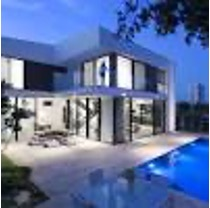
\includegraphics[scale=0.6]{../images/Picture5.jpg}
	%\end{center} 
\end{itemize}
\textbf{Services} \\ 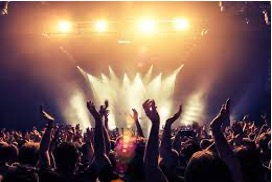
\includegraphics[scale=0.6]{../images/Picture6.jpg} 

\begin{itemize}
	\item{intangibles}
\end{itemize}

\begin{itemize}
	\item{And shift from manufacturing to services}
\end{itemize}

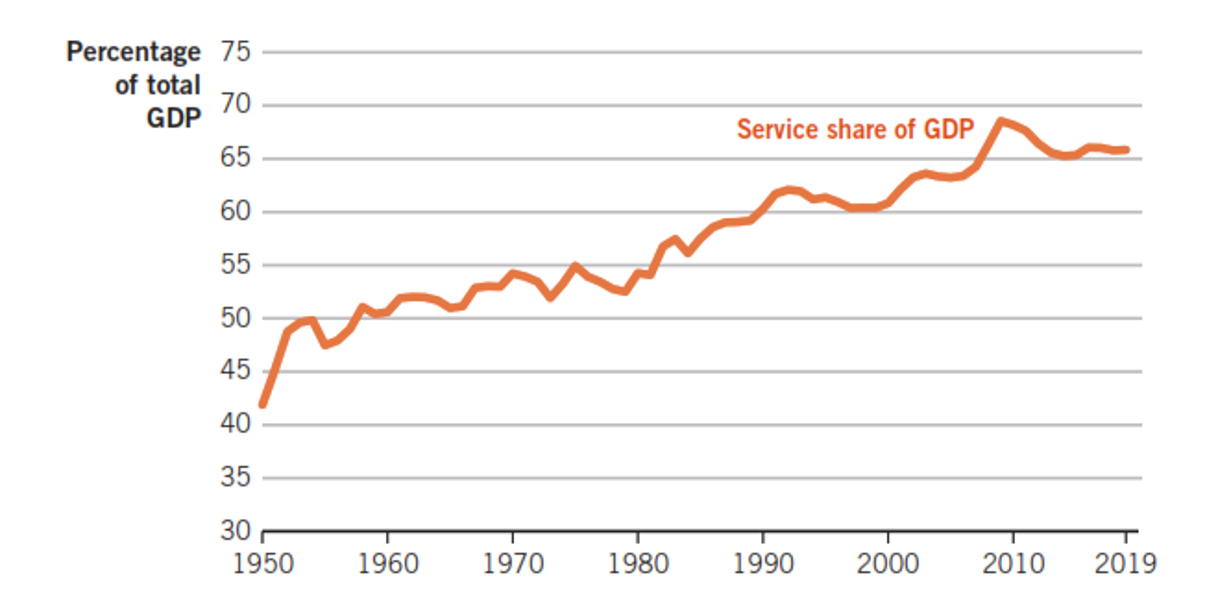
\includegraphics[scale=0.5]{../images/Picture7.png} 

\subsubsection*{Includes goods produced with a nation}
\subsubsection*{Gross National Product (GNP)}
Output produced by workers and resources owned by residents of the nation
\begin{itemize}
	\item{\textit{Nike shoes made in Thailand would count toward U.S's GNP but toward Thailand's GDP}}
\end{itemize}

\section{Four components of GDP}
The Bureau of Economic Analysis (BEA) is the U.S government agency that tallies GDP data, a task called national income accounting.
\begin{center}
\begin{equation}
Y=C+I+G+NX
\end{equation}
\begin{tabular}{|c|c|c|}
	\hline
	Y & Output \\
	\hline
	C & Consumption \\
	\hline
	I & Investment \\
	\hline
	G & Government Purchase \\
	\hline
	NX & Net Export \\
	\hline
\end{tabular}
\end{center}

Three types of investment is
\begin{enumerate}
	\item Investment
	\item Government Spending
	\item Net Exports \\
\end{enumerate}
Durable and non-durable goods; here are some examples.
\begin{itemize}
	\item Refrigerator
	\item Ice cream
	\item Shovel
\end{itemize}

\subsection{U.S GDP \& it's components (Example)}

\section{Calculating Real GDP}
\begin{itemize}
	\item Consider these 2 graphs. \\ 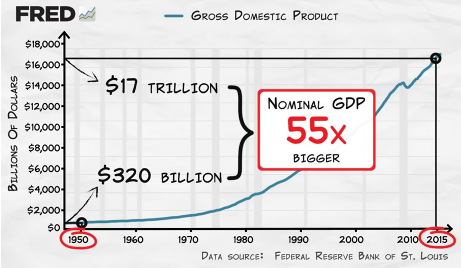
\includegraphics[scale=1]{../images/Picture2.png} \\ 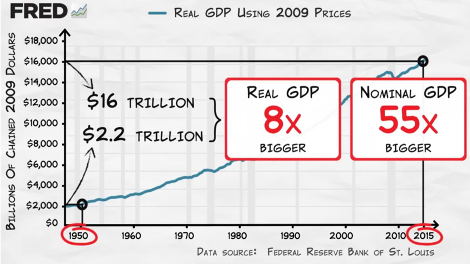
\includegraphics[scale=1]{../images/Picture3.png} 
	\item \textbf{Nominal GDP}
		\subitem{Can \(\Delta\) when P\(\Delta\), Q\(\Delta\), or both \(\Delta\)}
	\item \textbf{Real GDP}
		\subitem{Can only \(\Delta\) when Q\(\Delta\)}
\end{itemize}

\subsection{Nominal v. Real GDP}
\begin{itemize}
\item Nominal GDP
\subitem Value of the goods and services produced \textbf{current} prices
\item Real GDP
	\subitem Value of goods and services produced at \textbf{constant} prices
		\subsubitem Adjusted for inflation
\end{itemize}

\subsubsection*{Calculations}
\begin{center}
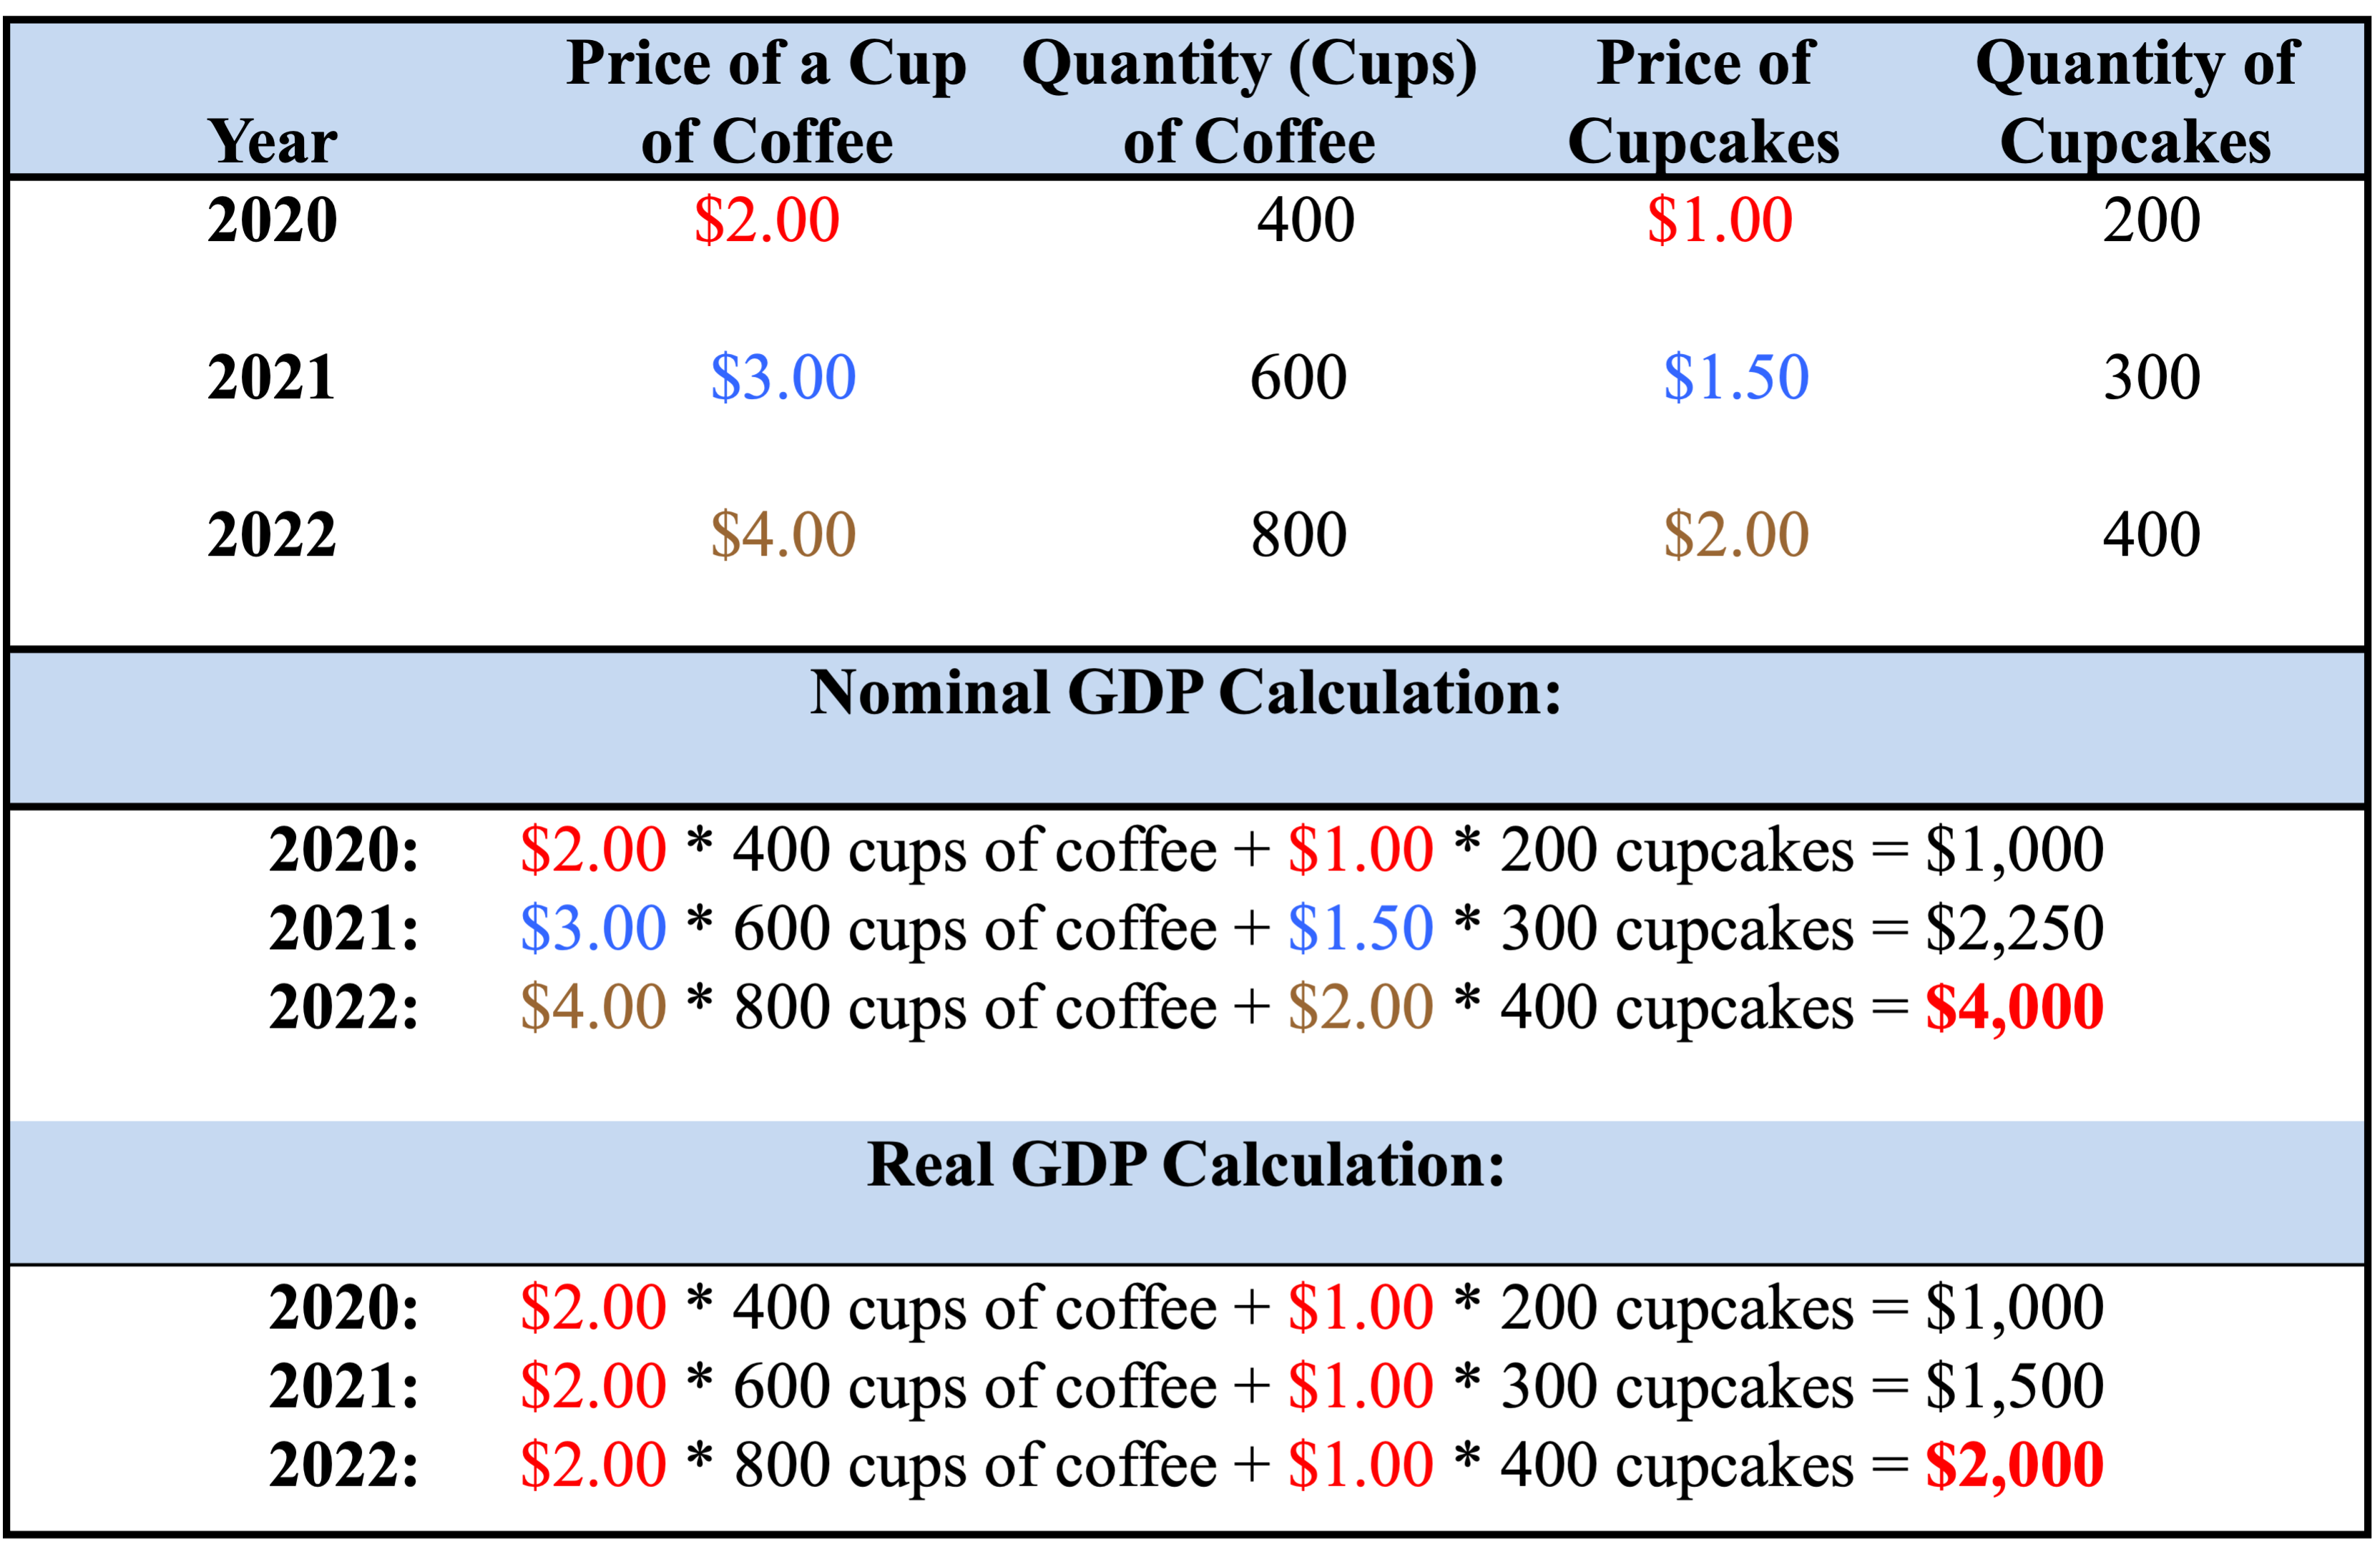
\includegraphics[scale=0.5]{../images/Picture10.png}
\end{center} 

\subsubsection*{U.S Nominal \& Real GDP}
\begin{center}
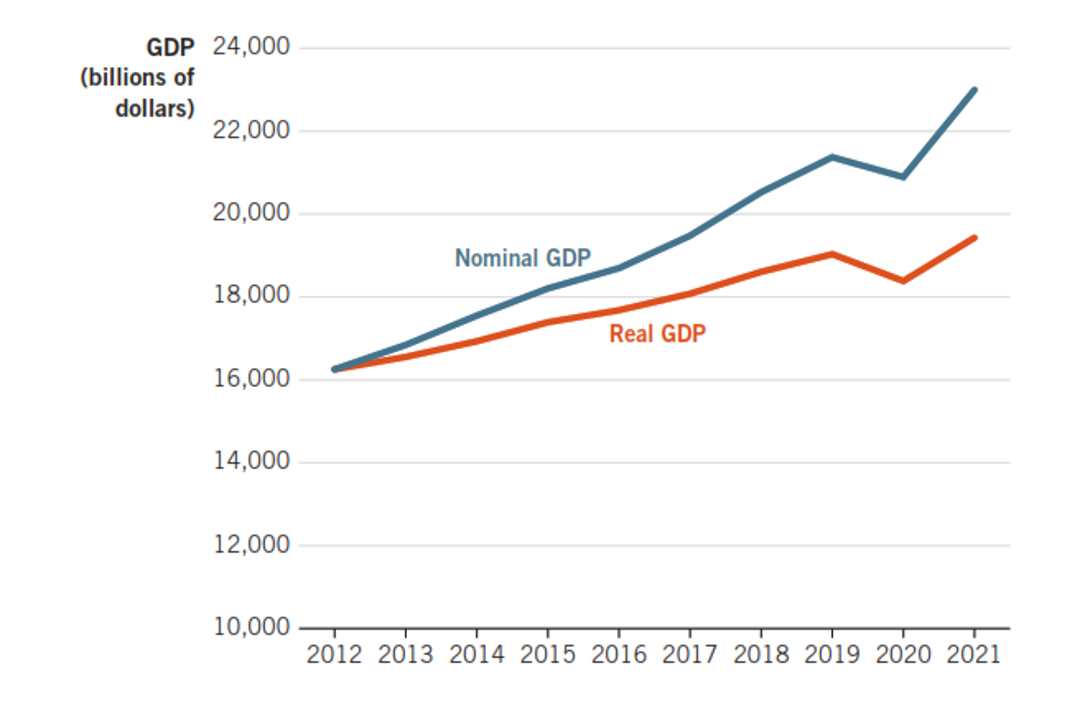
\includegraphics[scale=0.5]{../images/Picture9.png} 
\end{center}

\subsubsection*{Computing Real GDP}

\textbf{Two steps:}\\

\begin{enumerate}
\item Divide to filter out current prices.
\item Multiply to input base-period prices.
\end{enumerate}

\begin{equation}
\text{Real GDP}=\frac{\text{Nominal GDP}}{\text{Price Level}}\times 100
\end{equation}\\
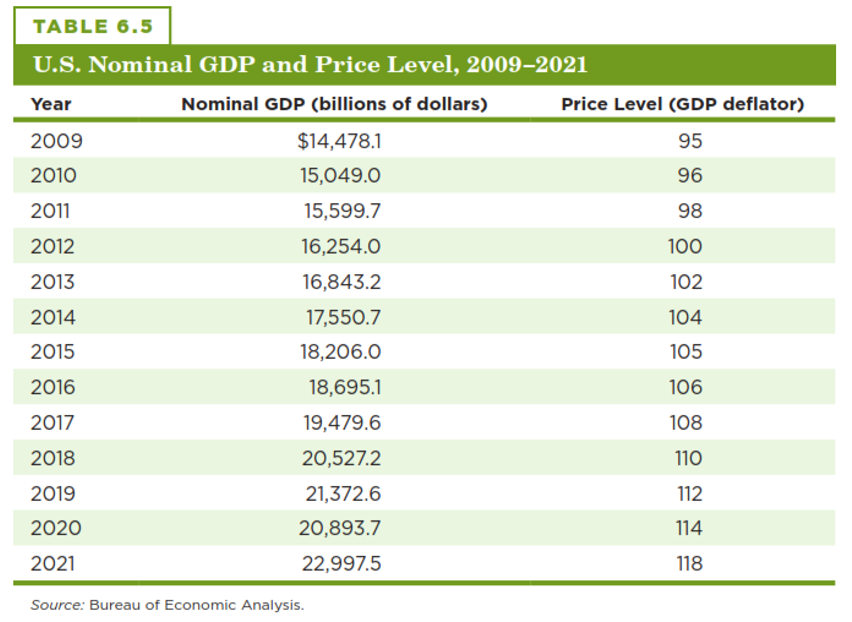
\includegraphics[scale=1]{../images/Picture11.png}\\
Compute 2021 real GDP in 2012 dollars for this graph.\\

\(\text{Real GDP}=\frac{22998}{118}\times 100=\$19,490 \;\text{billion}\)
\subsection{Three uses of GDP data}
\subsubsection{Growth Rates and Nominal GDP Growth Rate}
\begin{itemize}
\item GDP data can also be used to measure economic growth over time or changes in average living standards.
\item Economic growth - percentage change in real per capita GDP.
\item Have to adjust GDP for inflation.
\item The rate of change of nominal GDP from one year to the next \((\frac{\text{Value}_t-\text{Value}_{t-1}}{\text{Value}_{t-1}})\times 100\)
\item Where t is the current period value, and t-1 is the previous period value.
\item Can use this to calculate \% change in nominal GDP, price level, \& real GDP
\end{itemize}
\subsubsection{Measuring living standards}
\begin{itemize}
\item GDP offers us a way of estimating living standards across both time and place.
\item Does not take into account the population size of a country.
\item Have to adjust for population difference.
\item What is more desirable, a bigger GDP or a bigger GDP per capita.
\item \textbf{Per Capita GDP}
\subitem GDP per person
\item Measure of average living standards in a nation. \(\text{per capita GDP}=\frac{\text{GDP}}{\text{Population}}\)
\end{itemize}

\textbf{GDP does not fully account for:}
\begin{itemize}
\item Nonmarket goods
\item Underground economy
\item Quality of life
\item Leisure time
\item Distribution of income
\end{itemize}
\subsection{Shortcomings of GDP}
\begin{itemize}
\item Underground economy
\subitem Size of underground economy?
\subsubitem Percent of GDP (estimated) in United States
\subsubitem Percent in developing countries
\begin{center}
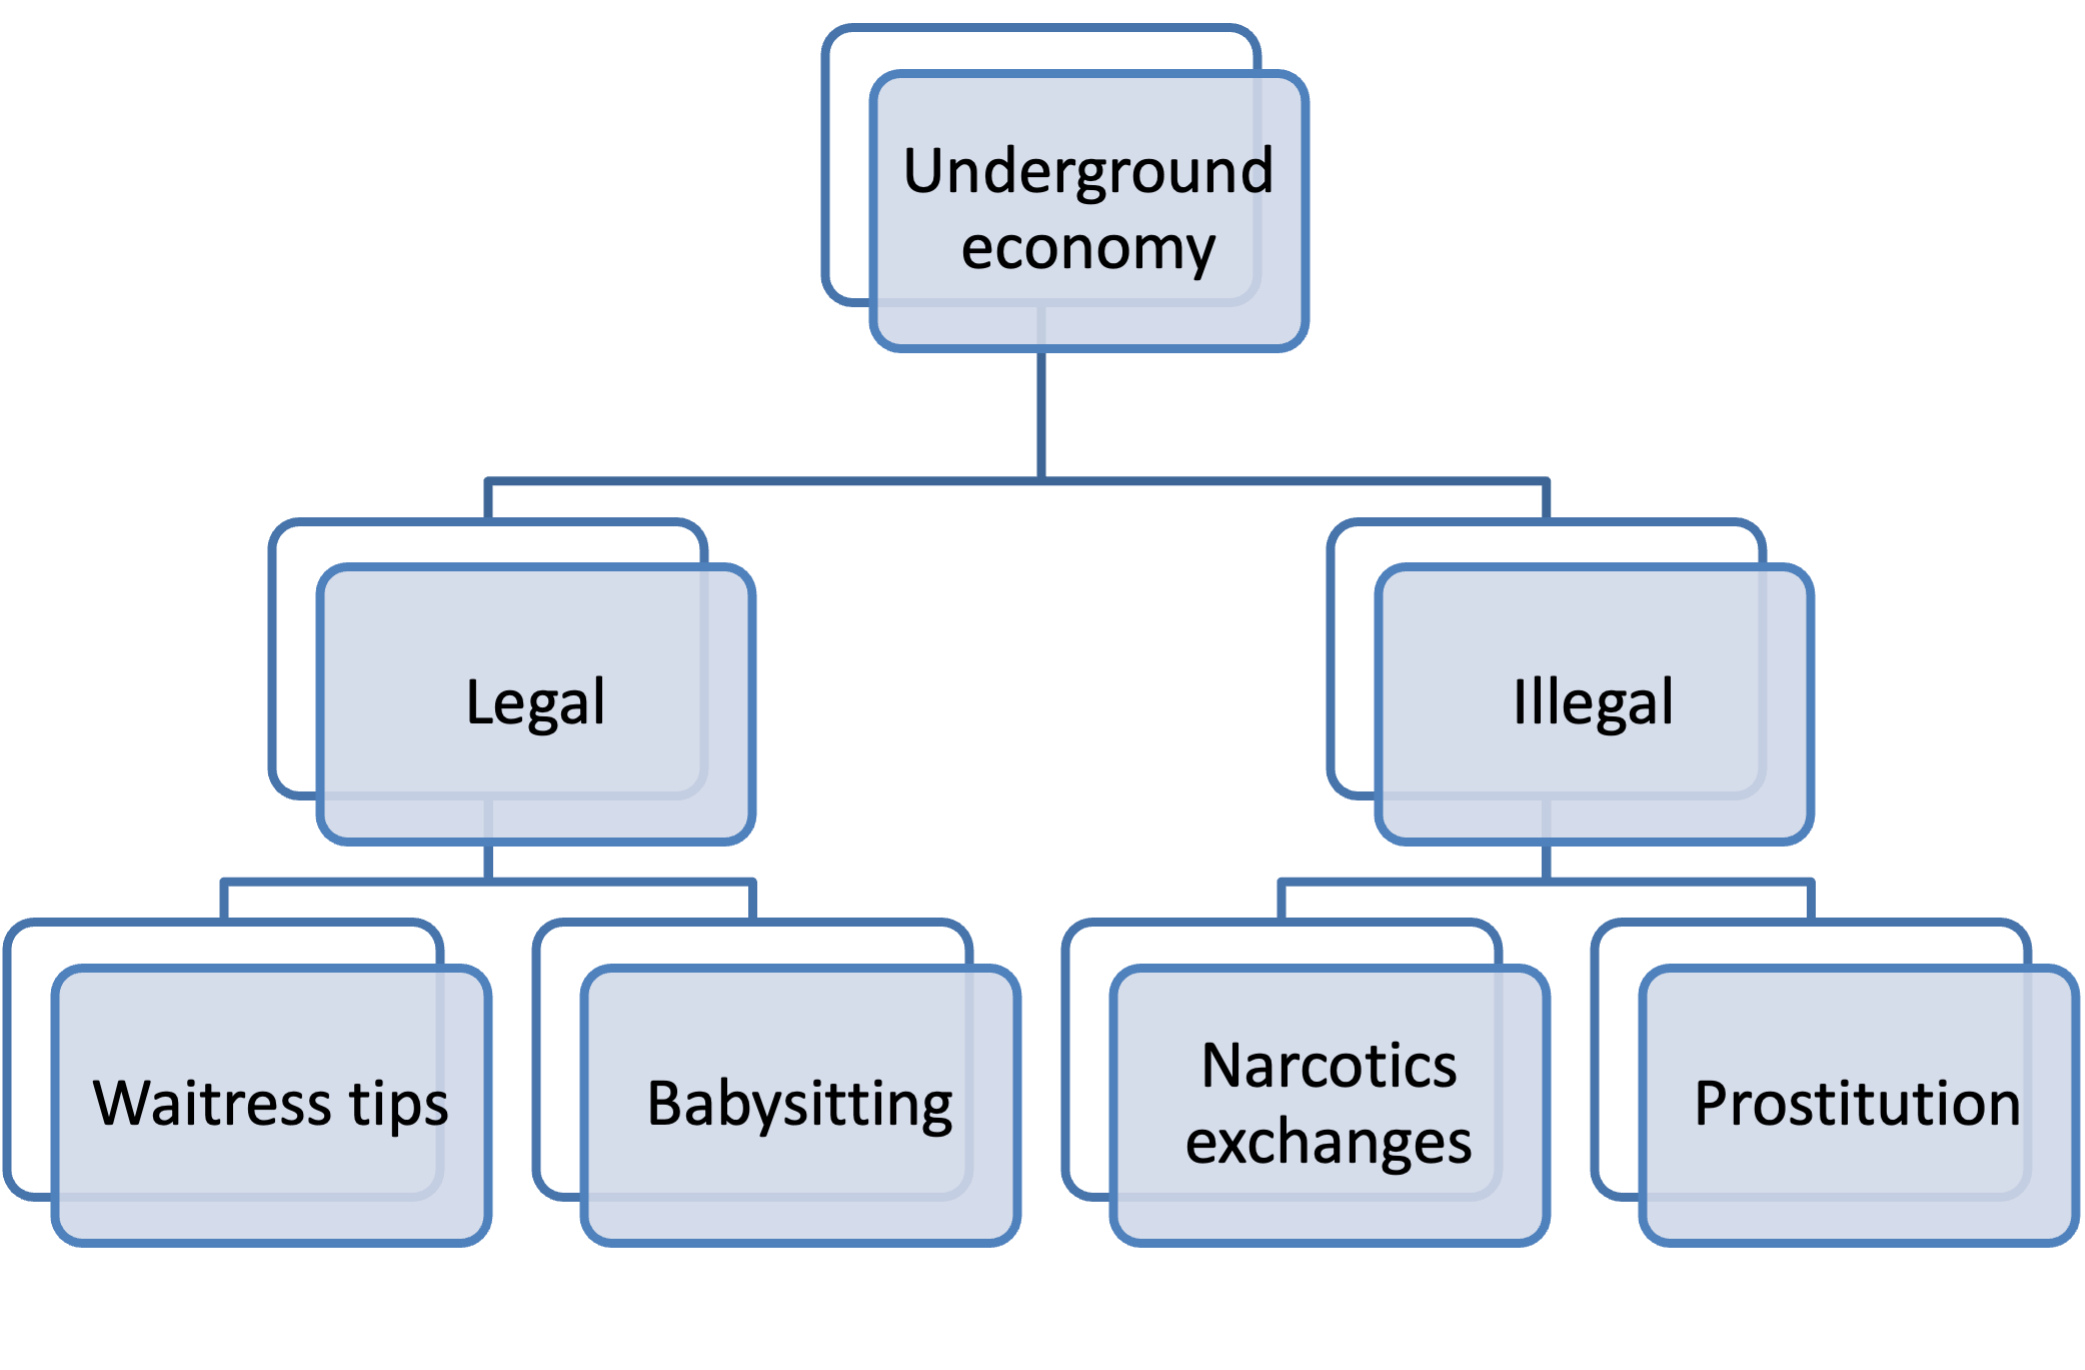
\includegraphics[scale=0.5]{../images/Picture14.png}
\end{center}
\end{itemize}

\subsection{GDP and the environment}
\begin{itemize}
\item When a factory sells goods, we count the goods in GDP.
\item When the factory hires a company to clean up the *blank* it creates, we also count that in GDP.
\item GDP *blank* the true value created.
\end{itemize}
\section{GDP = Happiness???}
\begin{itemize}
\item Life satisfaction is in nations with higher incomes.
\end{itemize}
\begin{center}
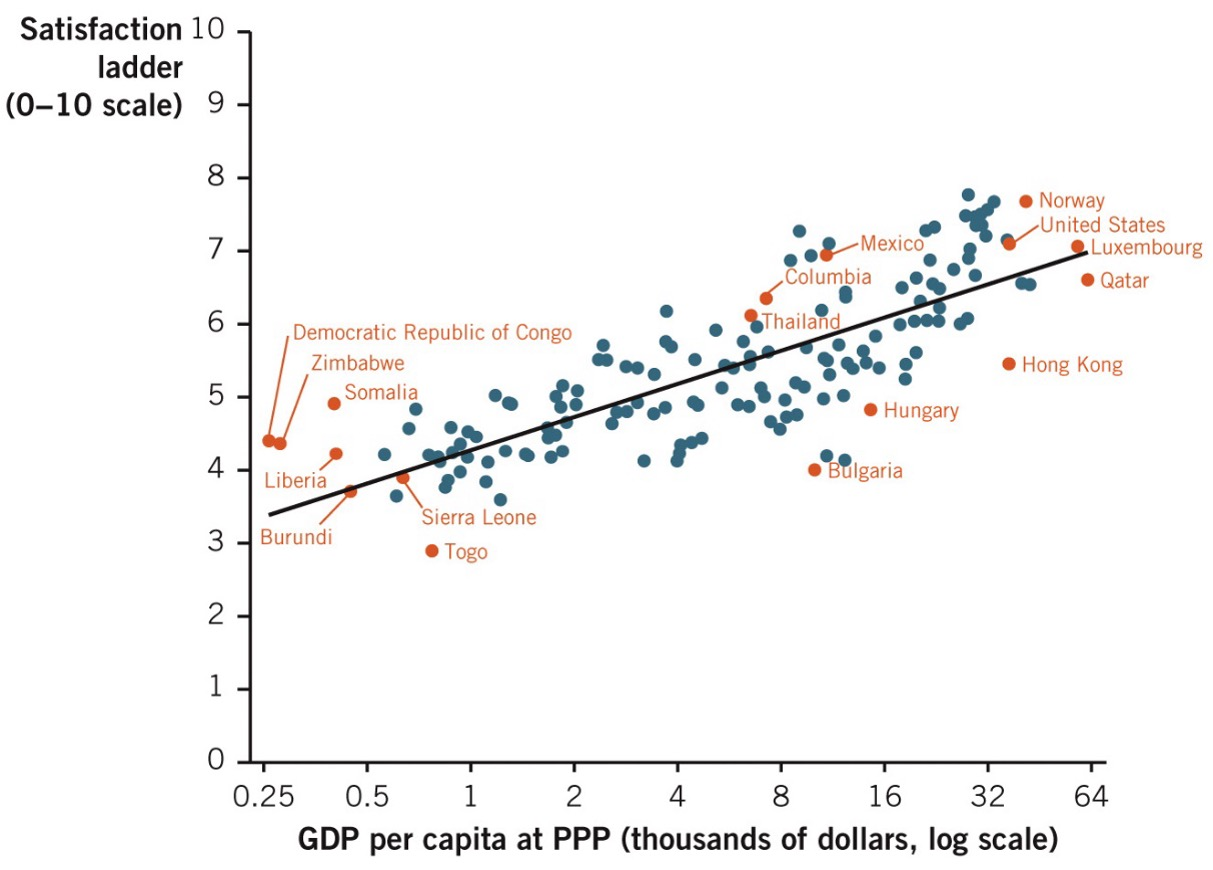
\includegraphics[scale=0.25]{../images/Picture15.jpg}
\end{center} 
In conclusion, higher income presents opportunities to pursue happiness.
\end{document}
